%% This is file `elsarticle-template-1-num.tex',
%%
%% Copyright 2009 Elsevier Ltd
%%
%% This file is part of the 'Elsarticle Bundle'.
%% ---------------------------------------------
%%
%% It may be distributed under the conditions of the LaTeX Project Public
%% License, either version 1.2 of this license or (at your option) any
%% later version.  The latest version of this license is in
%%    http://www.latex-project.org/lppl.txt
%% and version 1.2 or later is part of all distributions of LaTeX
%% version 1999/12/01 or later.
%%
%% The list of all files belonging to the 'Elsarticle Bundle' is
%% given in the file `manifest.txt'.
%%
%% Template article for Elsevier's document class `elsarticle'
%% with numbered style bibliographic references
%%
%% $Id: elsarticle-template-1-num.tex 149 2009-10-08 05:01:15Z rishi $
%% $URL: http://lenova.river-valley.com/svn/elsbst/trunk/elsarticle-template-1-num.tex $
%%
\documentclass[preprint,12pt]{elsarticle}

%% Use the option review to obtain double line spacing
%% \documentclass[preprint,review,12pt]{elsarticle}

%% Use the options 1p,twocolumn; 3p; 3p,twocolumn; 5p; or 5p,twocolumn
%% for a journal layout:
%% \documentclass[final,1p,times]{elsarticle}
%% \documentclass[final,1p,times,twocolumn]{elsarticle}
%% \documentclass[final,3p,times]{elsarticle}
%% \documentclass[final,3p,times,twocolumn]{elsarticle}
%% \documentclass[final,5p,times]{elsarticle}
%% \documentclass[final,5p,times,twocolumn]{elsarticle}

%% if you use PostScript figures in your article
%% use the graphics package for simple commands
%% \usepackage{graphics}
%% or use the graphicx package for more complicated commands
%% \usepackage{graphicx}
%% or use the epsfig package if you prefer to use the old commands
%% \usepackage{epsfig}

%% The amssymb package provides various useful mathematical symbols
\usepackage{amssymb}
%% The amsthm package provides extended theorem environments
%% \usepackage{amsthm}

%% The lineno packages adds line numbers. Start line numbering with
%% \begin{linenumbers}, end it with \end{linenumbers}. Or switch it on
%% for the whole article with \linenumbers after \end{frontmatter}.
%% \usepackage{lineno}

%% natbib.sty is loaded by default. However, natbib options can be
%% provided with \biboptions{...} command. Following options are
%% valid:

%%   round  -  round parentheses are used (default)
%%   square -  square brackets are used   [option]
%%   curly  -  curly braces are used      {option}
%%   angle  -  angle brackets are used    <option>
%%   semicolon  -  multiple citations separated by semi-colon
%%   colon  - same as semicolon, an earlier confusion
%%   comma  -  separated by comma
%%   numbers-  selects numerical citations
%%   super  -  numerical citations as superscripts
%%   sort   -  sorts multiple citations according to order in ref. list
%%   sort&compress   -  like sort, but also compresses numerical citations
%%   compress - compresses without sorting
%%
%% \biboptions{comma,round}

% \biboptions{}


\journal{Science of Computer Programming}

\usepackage{hyperref}
\usepackage{color}

\newcommand{\definition}[1]{ 
\begin{quote} \item {\em #1} \end{quote}}
\newcommand {\chaptersummary}[1] { \vspace{3cm} \hrule \vspace{0.5cm} {\em #1 } \vspace{0.5cm} \hrule \vspace{0.5cm} \newpage}
\newcommand{\challenge}[1]{\paragraph {\bf \em [Challenge]} {\em #1}} 



\newcommand{\chapquote}[1]{\em #1} 


\newcommand{\quest}[1]{{\em ({\bf Mircea:} #1)}}
\newcommand{\mir}[1]{{\em ({\bf Mircea:} #1)}}
\newcommand{\mircea}[1]{{\em ({\bf Mircea:} #1)}}
\newcommand{\Mircea}[1]{{\em ({\bf Mircea:} #1)}}

\newcommand{\pg}[2]{#1 #2}
%\newcommand{\pg}[2]{\paragraph {#1} {\small #2}}
\newcommand{\mic}[1]{{\small #1}}

\definecolor{lg}{rgb}{0.9,0.9,0.9}
\definecolor{darkblue}{rgb}{0.0,0.0,0.5}


\newcommand{\cbar}{\vspace {1cm} \hrule }

\newcommand{\concls}[1]{\titlebox{Facts and Limitations}{#1}}

\newcommand{\titlebox}[2]{
\vspace{1cm}
\hrule
\vspace{0.25cm}
{\bf #1: }
\vspace{0.25cm}
\hrule
#2
\vspace{0.5cm}
}


% Utils

\newcommand{\dpdef}[1]{\paragraph{Definition.} {\em #1}}
\newcommand{\dpdisc}[1]{\paragraph {Discussion.} #1}
\newcommand{\dpr}[1]{\paragraph {Rationale.} #1}
\newcommand{\dpcat}[1]{\paragraph {Category:} #1}
\newcommand{\dpcatage}{\dpcat{Age-related}}
\newcommand{\dpcatdyn}{\dpcat{Dynamics-related}}
\newcommand{\dpexample}[1]{\paragraph {Example.} #1}
\newcommand{\dpp}[1]{\newpage\subsection{#1}}


\newcommand{\pidea}[1]{#1.}
\newcommand{\pideap}[1]{#1}
%\newcommand{\pidea}[1]{\paragraph{#1.}}
%\newcommand{\pideap}[1]{\paragraph{#1} }



\newcommand{\flabel}[1]{\label{fig:#1}}
\newcommand{\tlabel}[1]{\label{tab:#1}}
\newcommand{\clabel}[1]{\label{c:#1}}
\newcommand{\slab}[1]{\label{sec:#1}}

\newcommand{\fref}[1]{Figure \ref{fig:#1}}
\newcommand{\tref}[1]{Table \ref{tab:#1}}
\newcommand{\sref}[1]{Section \ref{sec:#1}}
\newcommand{\cref}[1]{Section \ref{c:#1}}

% Font conventions
\newcommand{\partref}[2]{{\bf Part \ref{p:#1}: #2}}
\newcommand{\chap}[1]{\item {\bf Chapter \ref{c:#1}} {\footnotesize (p.\pageref{c:#1})}}
\newcommand{\apdx}[1]{\item {\bf Appendix \ref{c:#1}} {\footnotesize (p.\pageref{c:#1})}}
\newcommand{\spref}[1]{Section \ref{sec:#1} {\footnotesize (p.\pageref{sec:#1})}}

\newcommand{\SOC}{\subsubsection* {Structure of the Chapter}}

\newcommand{\q}[1]{``#1''}

\newcommand{\tool}[1]{{\em #1}}
\newcommand{\pnam}[1]{{\em #1}}
\newcommand{\trm}[1]{{\em #1}}

\newcommand{\art}[1]{{\em #1}}
\newcommand{\book}[1]{{\em #1}}
\newcommand{\cit}[1]{{\em ``#1''}}

\newcommand{\proj}[1]{{\em #1}}
\newcommand{\dev}[1]{{\em #1}}
\newcommand{\term}[1]{{\em #1}}
\newcommand{\class}[1]{{\em #1}}
\newcommand{\method}[1]{{\em #1}}
\newcommand{\met}[1]{{\em #1}}
\newcommand{\pack}[1]{{\em #1}}
\newcommand{\model}[1]{{\em #1}}
\newcommand{\vp}[1]{{\em #1}}

\newcommand{\metric}[1]{{\em #1}}

\newcommand{\cod}[1]{{\em #1}}



% Tables with metrics
\newcommand{\metrictableh}[4]{
\begin{table}[h!]
%\footnotesize
\centering
\begin{tabular}{l l}
#1
\hline
#2
\hline
\end{tabular}
\caption{#3}\tlabel{#4}
\end{table}
}

\newcommand{\metrictable}[3]{
\metrictableh
{Acronym & Name\\}{#1}{#2}{#3}
}




% viewpoint definitions
\newcommand{\vpc}{black}
\newcommand{\Goal}[1]{\subsubsection* {Goal} #1}
\newcommand{\Cat}[1]{\subsubsection* {Category} #1}

\newcommand{\Concerns}[1]{\paragraph{\textcolor{\vpc}{Concerns}} \begin{itemize}#1\end{itemize}}
\newcommand{\Stakeholders}[1]{\paragraph{\textcolor{\vpc}{Stakeholders: }} #1}
\newcommand{\Construction}[1]{\subsubsection* {Construction Principles } #1}
\newcommand{\Navigation}[1]{\paragraph{\textcolor{\vpc}{Implementation in SPO.}}  #1}
\newcommand{\Examples}{\subsubsection{\textcolor{\vpc}{Examples}}}
\newcommand{\Discussion}[1]{\subsubsection{\textcolor{\vpc}{Discussion}} 
\begin{description}
#1
\end{description}}
\newcommand{\dpoint}[1]{\item {\em #1.} }
\newcommand{\cpoint}[1]{\item {\bf #1.} }
\newcommand{\cpointnp}[1]{\item {\bf #1} }



% Frequently Used Terms
% ---------------------

\newcommand{\Revenge}{{Revenge}\xspace}
\newcommand{\revenge}{{revenge}\xspace}
\renewcommand{\v}{viewpoint\xspace}

% Generic 
\newcommand{\ie}{\textit{i.e.,}\xspace}
\newcommand{\eg}{\textit{e.g.,}\xspace}
\newcommand{\etc}{\textit{etc.}\xspace}
\newcommand{\etal}{\textit{et al.}\xspace}


% Super-repositories / Ecosystems
\newcommand{\super}{super-repository\xspace}
\newcommand{\Super}{Super-Repository\xspace}
\newcommand{\Supers}{Super-Repositories\xspace}
\newcommand{\supers}{super-repositories\xspace}
\newcommand{\spo}{Small Project Observatory\xspace}
\newcommand{\tspo}{The Small Project Observatory\xspace}
\newcommand{\snaut}{Softwarenaut\xspace}
\newcommand{\store}{Store\xspace}
\newcommand{\svn}{SVN\xspace}
\newcommand{\LEM}{{Lightweight Ecosystem Model}\xspace}
\newcommand{\emlem}{{\em lightweight ecosystem model}\xspace}
\newcommand{\lem}{{lightweight ecosystem model}\xspace}
\newcommand{\emdpm}{{\em detailed project model}\xspace}
\newcommand{\dpm}{{detailed project model}\xspace}
\newcommand{\DPM}{{Detailed Project Model}\xspace}

\newcommand{\treveale}{the REVEAL ecosystem \xspace}
\newcommand{\reveal}{{REVEAL}\xspace}
\newcommand{\scg}{{SCG}\xspace}
\newcommand{\cincom}{{Cincom}\xspace}
\newcommand{\soops}{{Soops}\xspace}
\newcommand{\gnome}{{Gnome}\xspace}


%~~~~~~~~~~
%Viewpoints 
%~~~~~~~~~~
 \newcommand{\growth}{{Size Evolution}\xspace}
 \newcommand{\vgrowth}{{Size Evolution}\xspace}
 \newcommand{\vgrowthv}{{Size Evolution} viewpoint\xspace}

 \newcommand{\vacti}{{Activity Evolution}\xspace}
 \newcommand{\vactiv}{{Activity Evolution} viewpoint\xspace}

 \newcommand{\vcol}{{Developer Collaboration}\xspace}
 \newcommand{\vcolv}{{Developer Collaboration} viewpoint\xspace}

 \newcommand{\varch}{{Project Architecture}\xspace}
 \newcommand{\varchv}{{Project Architecture} viewpoint\xspace}

 \newcommand{\vtimeline}{{Developer Timelines}\xspace}
 \newcommand{\vtimelinev}{{Developer Timelines} viewpoint\xspace}

 \newcommand{\vpdep}{{Project Dependency Map}\xspace}
 \newcommand{\vpdepv}{{Project Dependency Map} viewpoint\xspace}

 \newcommand{\vpmat}{{Project Dependency Matrix}\xspace}
 \newcommand{\vpmatv}{{Project Dependency Matrix} viewpoint\xspace}



%~~~~~~~~~~~~~~
% Soops report
%~~~~~~~~~~~~~~

\newcommand{\soopsPart}[1]{\subsubsection* {\em #1}}





%
\newcommand{\s}{Softwarenaut\xspace}
\newcommand{\shrimp}{SHriMP\xspace}

% Package Patterns 
\newcommand{\Autonomous}{Autonomous\xspace}
\newcommand{\FallThrough}{Fall-Through\xspace}
\newcommand{\Iceberg}{Iceberg\xspace}
\newcommand{\Archipelago}{Archipelago\xspace}
\newcommand{\vpsem}{{\em vertical package slices}\xspace}
\newcommand{\vps}{vertical package slices\xspace}
\newcommand{\Vps}{Vertical package slices\xspace}
\newcommand{\VPS}{Vertical Package Slices\xspace}
\newcommand{\VPSem}{{\em Vertical Package Slices}\xspace}

% Dependency Evolution Patterns
\newcommand{\sdm}{{\em Semantic Dependency Matrix}\xspace}
\newcommand{\refil}{Relationship Evolution Filmstrip\xspace}




% -----------------------------------------------

\hypersetup{
    bookmarks=true,         % show bookmarks bar?
    unicode=false,          % non-Latin characters in Acrobat’s bookmarks
    pdftoolbar=true,        % show Acrobat’s toolbar?
    pdfmenubar=true,        % show Acrobat’s menu?
    pdffitwindow=false,     % window fit to page when opened
    pdfstartview={FitH},    % fits the width of the page to the window
    pdftitle={Reverse Engineering Software Ecosystems},    % title
    pdfauthor={Mircea Lungu},     		% author
    pdfsubject={Doctoral Dissertation},   	% subject of the document
    pdfcreator={Mircea Lungu},   		% creator of the document
    pdfproducer={Mircea Lungu}, 		% producer of the document
    pdfkeywords={keywords}, 			% list of keywords
    pdfnewwindow=true,      			% links in new window
    colorlinks=true,       			% false: boxed links; 
    linkcolor=darkblue,          		% color of internal links
    citecolor=darkblue,        			% color of links to bibliography
    filecolor=magenta,      			% color of file links
    urlcolor=cyan           			% color of external links
}




\graphicspath{{images/}}

\begin{document}


\begin{frontmatter}

%% Title, authors and addresses

%% use the tnoteref command within \title for footnotes;
%% use the tnotetext command for the associated footnote;
%% use the fnref command within \author or \address for footnotes;
%% use the fntext command for the associated footnote;
%% use the corref command within \author for corresponding author footnotes;
%% use the cortext command for the associated footnote;
%% use the ead command for the email address,
%% and the form \ead[url] for the home page:
%%
%% \title{Title\tnoteref{label1}}
%% \tnotetext[label1]{}
%% \author{Name\corref{cor1}\fnref{label2}}
%% \ead{email address}
%% \ead[url]{home page}
%% \fntext[label2]{}
%% \cortext[cor1]{}
%% \address{Address\fnref{label3}}
%% \fntext[label3]{}

\title{Softwarenaut:\\ Explorative Software Architecture Recovery}


%% use optional labels to link authors explicitly to addresses:
%% \author[label1,label2]{<author name>}
%% \address[label1]{<address>}
%% \address[label2]{<address>}

\author{Mircea Lungu}
\address{Software Composition Group - University of Bern, Switzerland}

\author{Michele Lanza}
\address{REVEAL @ Faculty of Informatics - University of Lugano, Switzerland}


\begin{abstract}
When the initial architecture of a system has eroded the only solution is architecture recovery. However, when the system under analysis is large, the user must use dedicated tools to support the recovery process. In this article we present Softwarenaut -- a tool which supports architecture recovery through interactive exploration and visualization. The tool provides overview and detailed perspectives which support the architecture recovery process as well as powerful navigation primitives and filtering mechanisms that allow managing the complexity of large software systems. The recovered architectural views can be shared between users through a Global Architectural View Repository allowing collaborative architecture recovery.
\end{abstract}

\begin{keyword}
Architecture Recovery \sep Visualization \sep Reverse Engineering
\end{keyword}

\end{frontmatter}

%%
%% Start line numbering here if you want
%%

%%%%%%%%%%%%%%%%%%%%%%
%%%%%%%%%%%%%%%%%%%%%%
\section{Introduction} \label{sec:Introduction}
%%%%%%%%%%%%%%%%%%%%%%
%%%%%%%%%%%%%%%%%%%%%%

No software system is an island. Instead a system exists and functions in an environment, and when the environment changes the system must change too or become obsolete\cite{lehman-softev}. As a result, maintaining a software system implies a continuous effort to keep it up to date with the unanticipated changes in its environment. Having a clear and up to date understanding of the architecture of a system is critical for its maintenance and evolution \cite{Duca09c, pollet-sar}.

As a system evolves, the architecture erodes \cite{perry-foundations} and an architectural mismatch appears between the {\em as-defined} and {\em as-is} architecture \cite{garlan-mismatch}. One accompanying property of this continuous drift between the actual architecture and the defined architecture of the system is an increasing brittleness of the system \cite{perry-foundations}. The main reason for architectural erosion and drift is widespread lack of programming language support for expressing the architecture, as well as the lack of tools that associate architectural decisions with the source code. The problem is an instance of the documentation problem: it is well known that the documentation of the system becomes quickly obsolete unless developers dedicate conscientious effort towards keeping it up to date \cite{riva-report}.

When the drift and erosion have brought the system architecture too far from the initial state, the solution is to recover the architecture of the system from the source code. Jazayeri defined architecture recovery as ``{\em the techniques and processes used to uncover a system's architecture from available information}'' \cite{jaza-archevo}. 

In the case of large software systems the architecture is specified through multiple architectural views that correspond to a set of given {\em architectural viewpoints}. An architectural viewpoint is a pattern or template from which to develop individual views by establishing the purposes and audience for a view and the techniques for its creation and analysis. Even if different authors propose different viewpoints \cite{bass-architecture, kruchten-4plus, hof-apparch} the consensus is that multiple viewpoints are necessary for capturing all the various facets of a system.

Usually, architecture recovery tools focus on recovering module views through visualization and interaction \cite{murphy-reflexion, muller-rigi, storey-shrimp}. While some steps of the process can be automated (e.g., fact extraction, view generation), no tool works completely without human intervention. In some cases the user has to group related artifacts together based on their similarity of purpose \cite{muller-rigi}. In other cases the user has to compare the architecture as-extracted with the architecture as-predicted \cite{murphy-reflexion} or the user has to decide which exploration paths to follow \cite{storey-shrimp}.

We present Softwarenaut \cite{lungu-relevo, lungu-packages} - the architecture recovery tool that we have developed. Softwarenaut provides interactive exploration mechanisms that support the semi-automated discovery of architectural views of any object-oriented system and allows the sharing of such architectural views. 

{
%\footnotesize 
\paragraph{Structure of the article} \sref{over} is an overview of Softwarenaut. The following two sections discuss two important phases in the workflow of any architecture recovery tool: information aggregation (\sref{org}) and interactive exploration (\sref{interact}). In \sref{archi} we discuss architectural considerations and in \sref{disc} we discuss the tool-building experience. In \sref{rel} we present related work. In \sref{conc} we conclude and outline future directions.

}
%%%%%%%%%%%%%%%%%%%%%%%%%%%%%%%%%%%%%
%%%%%%%%%%%%%%%%%%%%%%%%%%%%%%%%%%%%%
\section {Softwarenaut in a Nutshell} \label{sec:over}
%%%%%%%%%%%%%%%%%%%%%%%%%%%%%%%%%%%%%
%%%%%%%%%%%%%%%%%%%%%%%%%%%%%%%%%%%%%

Softwarenaut is an architecture recovery tool based on interactive exploration, with the goal of discovering architecturally relevant views \cite{lungu-packages}.

The main interaction approach in Softwarenaut is to let the user navigate from an automatically aggregated high-level view on the system downwards, also known as {\em top-down exploration}.


\begin{figure}[h]
\begin{center}
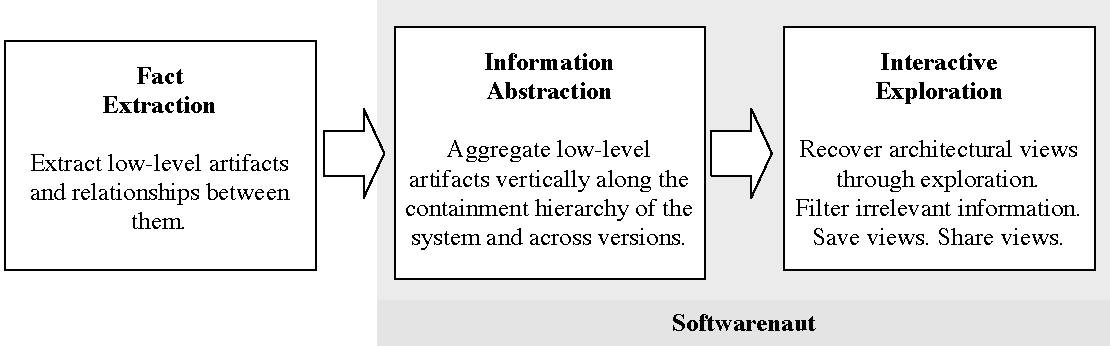
\includegraphics[width=\linewidth]{SnautWorkflow}
\caption{Softwarenaut supports an extract-abstract-view workflow model}
\flabel{flow}
\end{center}
\end{figure}

Like other architecture recovery tools \cite{pollet-sar}, Softwarenaut conforms to a classical extract-abstract-view architecture. \fref{flow} presents the three main steps of this architecture. In each of the three steps the tool offers state of the art features:

\begin{itemize}
\item {\em Fact Extraction.} The tool can analyze any object-oriented system through a system of pluggable fact extractors which export information to a well-known meta-model. 
\item {\em Information Aggregation.} The tool takes into account the hierarchical decomposition of a system as a basis for aggregating artifacts and relationships. In the case of a missing hierarchical decomposition the tool can automatically generate one.
\item {\em Interactive Visualization and Exploration.} The tool allows for an overview, zoom and filter, and details on demand approach. The tool provides a powerful set of filtering mechanisms. The recovered architectural views can be shared between users, and reused by other tools.
\end{itemize}
%, {\em fact extraction}, {\em information aggregation}, and {\em interactive visualization and exploration}.

The article continues with detailing the second and third step, the first one being discussed later in the section on architectural concerns regarding the tool.



%%%%%%%%%%%%%%%%%%%%%%%%%%%%%%%%%%%%%
%%%%%%%%%%%%%%%%%%%%%%%%%%%%%%%%%%%%%
\section {Information Abstraction} \label{sec:org}
%%%%%%%%%%%%%%%%%%%%%%%%%%%%%%%%%%%%%
%%%%%%%%%%%%%%%%%%%%%%%%%%%%%%%%%%%%%

Aggregating horizontal relationships between software artifacts along the containment relationships is the fundamental technique that enables abstraction in Softwarenaut. 

\fref{dep-agg} exemplifies the aggregation of low-level relationships between methods and classes along the containment hierarchy of a Java system. 

\begin{figure}[ht]
\begin{center}
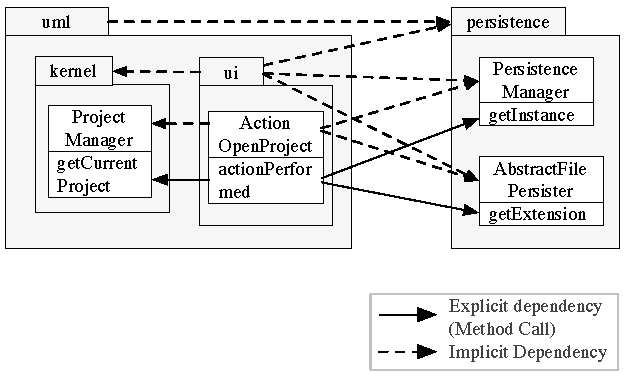
\includegraphics[width=0.9\linewidth]{DependencyAggregation}
\caption{The aggregation of explicit dependencies into implicit ones along the containment relationships between methods, classes, and packages in a Java system}
\flabel{dep-agg}
\end{center}
\end{figure}

The example contains two explicit low-level dependencies: the method calls between \cod{mc1} and respectively \cod{mc2} and \cod{mc5}. The explicit dependencies propagate as implicit relationships vertically along the containment relationships \cod{mc1 $\rightarrow$ c1 $\rightarrow$ B  $\rightarrow$A}, \cod{mc5 $\rightarrow$ c5 $\rightarrow$ d $\rightarrow$ c} and \cod{mc2 $\rightarrow$  c2 $\rightarrow$  d $\rightarrow$ c}. The highest level implicit relationship is the one between A and C. 

A data structure that allows for this is the Higraph introduced by Harel \cite{harel-visform}. In our case, the DPMHigraph\footnote{DPM stands for Detail Project Model. For the importance of the concept see  \cite{lungu-thesis}} is a data structure formed by taking the graph of basic artefacts and relationships between them and aggregating them along the containment hierarchy of the system. 

\begin{figure}[h]
\begin{center}
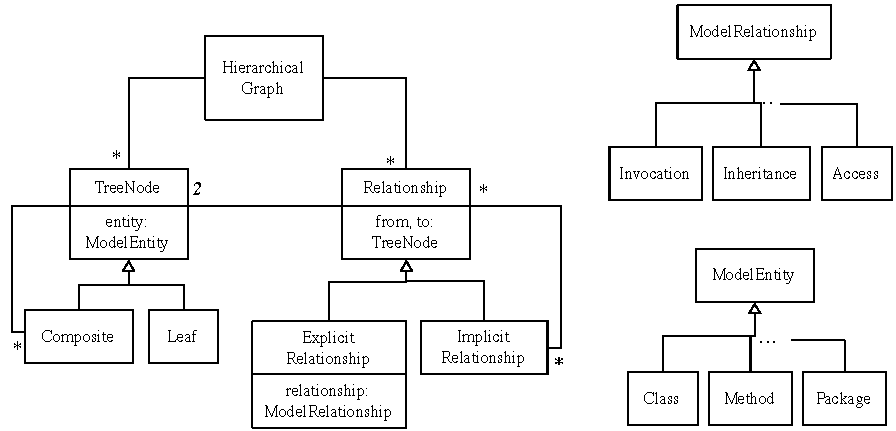
\includegraphics[width=0.9\linewidth]{HigraphModel}
\caption{The DPMHigraph model is the core representation of a system in Softwarenaut}
\flabel{hmodel}
\end{center}
\end{figure}

The diagram from \fref{hmodel} presents two types of abstract entities and two types of abstract relations:

\begin{itemize}

\item {\em Leaf Entities}. They are the basic object-oriented programming building blocks used for the structuring of software. Depending on the analyzed relationship, the leaf entities can be either methods or classes.

\item {\em Composite Entities}. The composite entities are containers for other entities. They can have direct mappings to programming language entities, such as classes, packages, namespaces or modules but can also represent abstract composites such as clusters.

\item {\em Explicit Relationships}. These are the relations between two entities as they exist in the code. Softwarenaut models method invocations, class inheritance, and field access.

\item {\em Implicit Relationships}. The model admits relationships between any abstract entities. However, in software systems explicit relationships usually exist only between the leaf entities. Therefore, the relations between the composite entities must be inferred bottom-up from the relations existing between the leafs. The result is that between any two high-level components, we have a relation that represents a collection of all the relations between the leaf components aggregated in them.

\end{itemize}


\newpage
%%%%%%%%%%%%%%%%%%%%%%%%%%%%%%%%%%%%%
%%%%%%%%%%%%%%%%%%%%%%%%%%%%%%%%%%%%%
\section {Interactive Exploration} \label {sec:interact}
%%%%%%%%%%%%%%%%%%%%%%%%%%%%%%%%%%%%%
%%%%%%%%%%%%%%%%%%%%%%%%%%%%%%%%%%%%%
The UI of Softwarenaut contains three linked complementary visual perspectives that present information about a system during the exploration. \fref{sos} presents Softwarenaut visualizing an architectural view of itself. The linked complementary perspectives support the ``overview first, zoom and filter, and details on demand'' principle of information visualization \cite{shneid-eyes}. 



\begin{figure}[ht]
\begin{center}
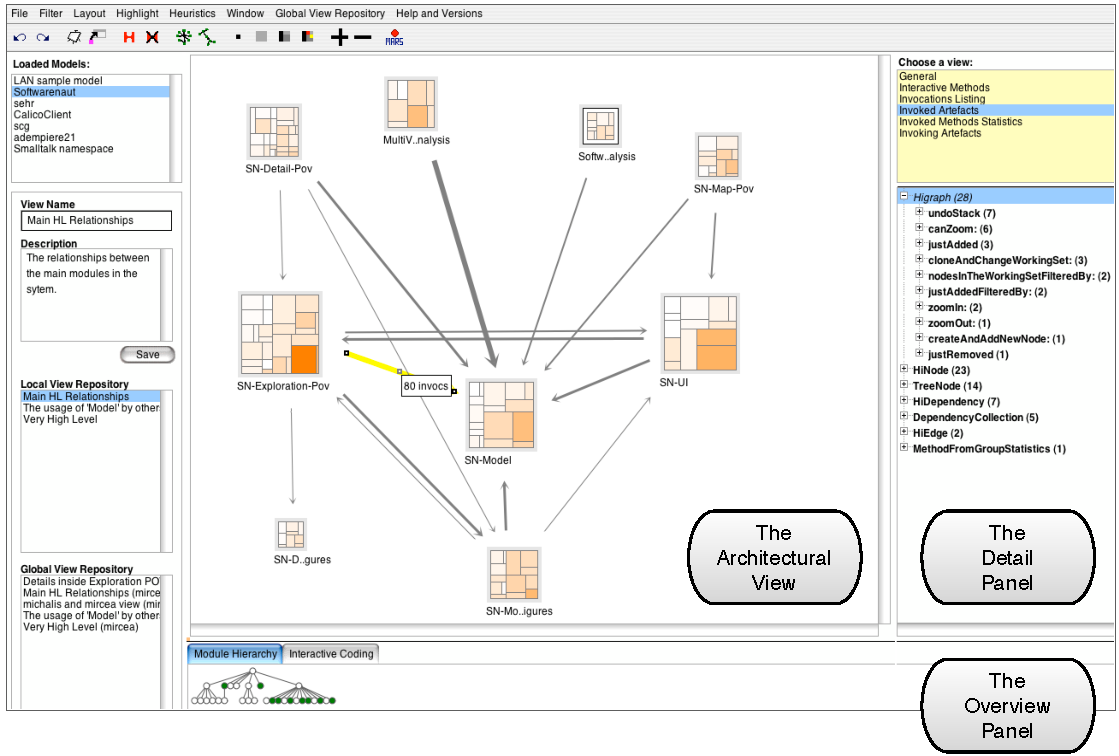
\includegraphics[width=\linewidth]{SnautOnSnaut.pdf}
\caption{Linked views present complementary perspectives on a software system }
\flabel{sos}
\end{center}
\end{figure}

The three complementary views that the tool supports:

\begin{enumerate}

\item The {\em Exploration} panel is Softwarenaut's main view. It is a graph-based representation of modules and their dependencies. The nodes in the graph represent modules and the edges represent the dependencies between the modules. Each dependency edge is an aggregation of low-level dependencies between the two associated modules. To represent the nodes and edges here we use Lanza's polymetric approach \cite{lanza-pv, lanza-oomp}. 

\item The {\em Detail} panel presents details for an entity selected in the Exploration panel. The goal is to supplement details of the element selected in the exploration panel. The detail panel implements the ``details-on-demand'' part of Shneiderman's visualization mantra \cite{shneid-eyes}.

\item The {\em Overview} panel presents the entire hierarchy of a system and highlights the modules that are visible in the exploration panel. The Overview panel presents a horizontal slice through a system \cite{wong-thesis}, offering an orientation aid which is critical for successful navigation \cite{storey-awareness}.

\end{enumerate}

In this section we detail the interactive techniques that support the exploration process in Softwarenaut: navigation (\ref{sec:navi}), details-on-demand (\ref{sec:dod}), rule-based filtering (\ref{sec:filtering}) and first-class views and collaboration (\ref{sec:views}).  

%%%%%%%%%%%%%%%%%%%%%%%%%%%%%%%%%%%%%
\subsection{Navigation} \slab{navi}
%%%%%%%%%%%%%%%%%%%%%%%%%%%%%%%%%%%%%

The dominant exploration mechanism of Softwarenaut is navigation along the vertical decomposition of the system. One starts with a very high-level abstracted view of a system and continuously refines by using exploration operations \cite{robertson-conetrees}. At any given moment the set of visible nodes in the exploration view with which the user interacts constitutes the working set (WS). Initially the working set contains very few high-level nodes. As the user explores the system he transforms the working set by performing exploration operations on it and thus changes the contents of the view in the exploration view.

\begin{figure}[ht]
\begin{center}
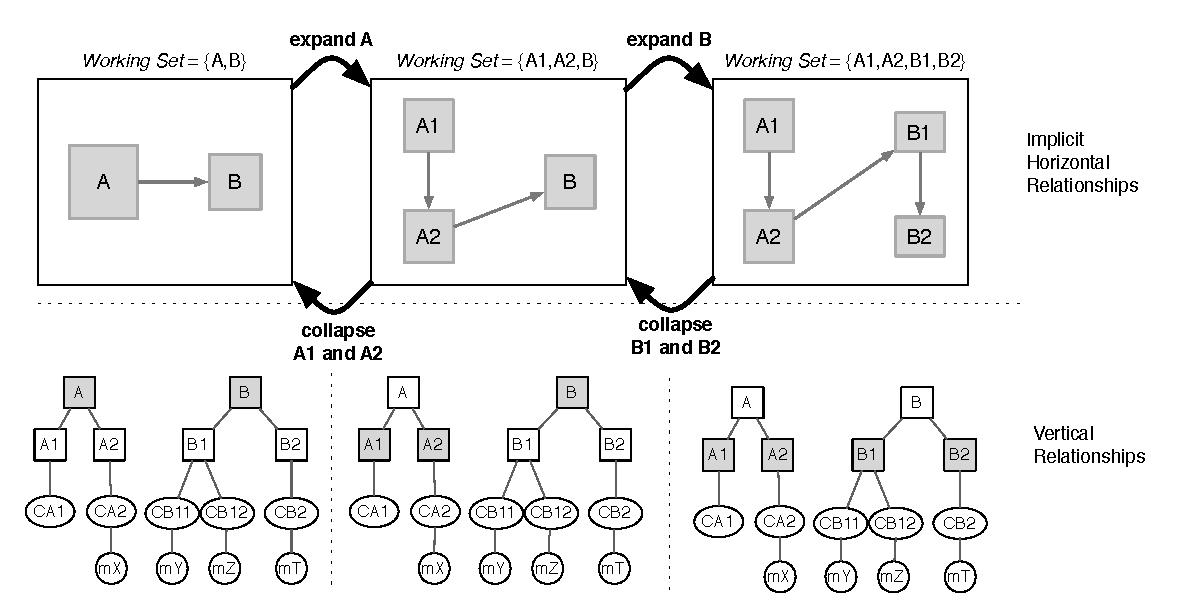
\includegraphics[width=\linewidth]{SnautSequence}
\caption{The expand and collapse complementary operations that allow vertical navigation in the Higraph}
\label{}
\end{center}
\end{figure}

The exploration operations supported by Softwarenaut are:

\begin{itemize}

\item {\em Expand}. The expand operation applied to a node of the working set replaces in the working set the node with nodes that represent its children. We define the operation formally as follows: 

$ Expand_{N,HG} (WS) = WS - N + children (N, HG)$, 

where $children(x,h)$ is a function which returns the children of node $x$ in higraph $h$.

\item {\em Collapse}. The collapse operation applied to a module in the working set removes the module and all its siblings from the view and replaces them with their parent module. We define the operation as follows:

$ Collapse_{N,HG} (WS) = WS - N - siblings (N, HG) + parent (N, HG)$

where $siblings(x,h)$ is a function which returns the nodes that have the same parent with $x$ in higraph $h$, and $parent(x,h)$ is a function which returns the parent of node $x$ in higraph $h$. 

\item {\em Filter}. The filter operation applied to a node removes that node from the working set. We define the operation as follows:

$ Filter_{N,HG} (WS) = WS - N$

\item {\em Group}. The group operation applied to several modules removes the modules from the view and replaces them with a new virtual module. By grouping several modules together the user reduces the clutter in the view. We define the group operation as follows: 

$ Group_{N_{i},HG} = WS - N_i + NewGroupNode $

where $N_i$ is the set of nodes the user wants to group.

\end{itemize}

As the user refines the view, and climbs down in the hierarchy of the system, he brings more and more elements into the view. He can use the Filter and Group operations on explicit sets of nodes to decrease the number of nodes displayed on screen and therefore cope with the complexity of large graphs. One type of modules that benefit the user when filtered out are the {\em omnipresent modules} which contribute little to the understanding of the architecture of the system, and heavily clutter the view \cite{mitchell-bunch}.

%%%%%%%%%%%%%%%%%%%%%%%%%%%%%%%%%%%%%
\subsection {Details-on-Demand} \slab{dod}
%%%%%%%%%%%%%%%%%%%%%%%%%%%%%%%%%%%%%

The elements of every architectural view in Softwarenaut are nodes that represent modules and edges that represent relationships between them. For the user to be confident that he {\em understands} such a view he needs to understand the role of every node and the meaning of every edge. Metaphorically, if the view were a phrase, the nodes would be the nouns and the edges would be the verbs. Only when one has understood all the nouns and the verbs he has really understood the story of the view.  

The Detail panel of Softwarenaut is one of the ways in which one can understand the individual nodes and edges in an architectural view; it presents different views depending on the selected element in the exploration view. 

%%%%%%%%%%%%%%%%%%%%%%%%%%%%%%%%%%%%%
\subsubsection {Detail Views for Modules}
%%%%%%%%%%%%%%%%%%%%%%%%%%%%%%%%%%%%%

The detail views for modules present various aspects of a selected module. \fref{dnode} presents the {\em Class Metrics} detail view which lists all the classes contained in a module together with a customizable set of metrics for them.

\begin{figure}[ht]
\begin{center}
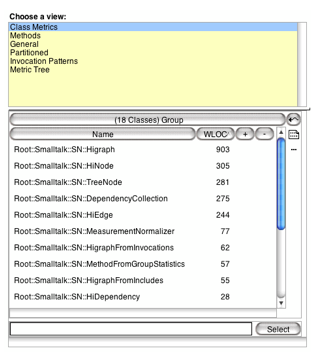
\includegraphics[width=0.55\linewidth]{DetailForNode}
\caption{The Class Metrics view shows the list of classes in a module. The classes are sorted based on their size and the user can navigate to the source of individual classes.}
\flabel{dnode}
\end{center}
\end{figure}

%%%%%%%%%%%%%%%%%%%%%%%%%%%%%%%%%%%%%
\subsubsection {Detail Views for Relationships}
%%%%%%%%%%%%%%%%%%%%%%%%%%%%%%%%%%%%%

The detail views for relationships present information about the selected relationships. Since understanding the relationships is critical for understanding the view, Softwarenaut provides a broad set of detail views for relationships which cover both structural and evolutionary aspects of the relationships \cite{lungu-cutedge, lungu-relevo}. \fref{dedge} presents two such interactive detail views: 

\begin{description}
\item The {\em Invoked Artefacts} view lists all the artefacts invoked by the selected high-level dependency. The tree has on its first level the invoked classes, on the second level invoked methods, and on the third level call sites. The user can navigate to any of the presented code artifacts from this view.
\item The {\em Evolution Filmstrip} view presents the evolution of the given relationship in all the versions of the system which are available for analysis \cite{lungu-relevo}. The two modules and the associated relationship are represented in every analyzed version. \fref{dedge} shows a relationship which changed dramatically during the six versions of the system under analysis. 
\end{description}

\begin{figure}[t]
\begin{center}
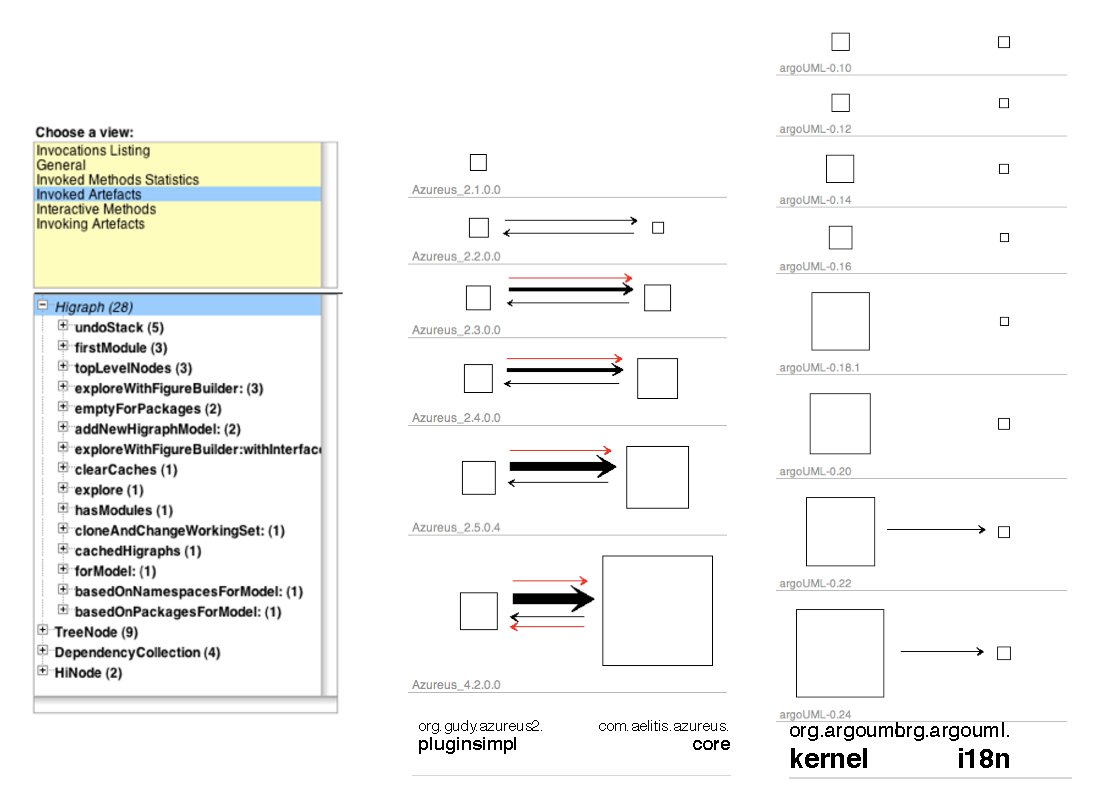
\includegraphics[width=0.8\linewidth]{DetailsForEdge}
\caption{Relationship details: Invoked Artifacts (left) and Evolution Filmstrip (right)}
\flabel{dedge}
\end{center}
\end{figure}



\newpage
\subsection {Rule-Based Filtering}
\slab{filtering}

In the previous section we have introduced the Filter operation which works on explicit sets of nodes. Most software architecture recovery tools offer such a filter operation \cite{aracic-filtering}. Softwarenaut implements several categories of advanced {\em rule-based filters} for nodes and edges. Softwarenaut supports two types of basic filters: 

\begin{enumerate}

\item {\em Low-level filters} act on the higraph itself. They remove from the higraph the low-level elements that match a given condition, e.g., all the invocation relationships that go to polymorphic classes.

\item {\em High-level filters} act on the high-level elements and relationships between them in the working set, e.g., hiding all the high-level dependencies that abstract few low-level dependencies.

\end{enumerate}

During exploration, the user interacts mostly with the High-level filters. There are two types of filters that apply to both artifacts and relationships: 

\begin{enumerate}
\item {\em Metric-based filters} for entities and relationships are defined with respect to the metrics computed for artifacts. For example filtering out {\em the weak dependencies} or {\em the small modules} in a view.
\item {\em Type-based filters} for entities and relationships are defined with respect to the type of the artifacts. For example showing {\em only inheritance relationships} or hiding {\em all the classes} from a view.
\end{enumerate}

Softwarenaut also implements advanced filters for relationships:

\begin{itemize}

\item {\em Evolutionary filters} are defined based on the historical evolution of an inter-module relationship in the system\footnote{Evolution-based filters require models of multiple versions of a system loaded}. For example showing only the {\em relationships that existed in all the versions of a system} or hiding all the {\em unstable relationships} \cite{lungu-relevo}.

\item {\em Directional filters} are defined based on the direction of the relationship between two modules. For example, filtering out the unidirectional relationships from an architectural view is useful for highlighting the modules that have mutual dependencies between themselves. 

\end{itemize}

\begin{figure}[ht]
\begin{center}
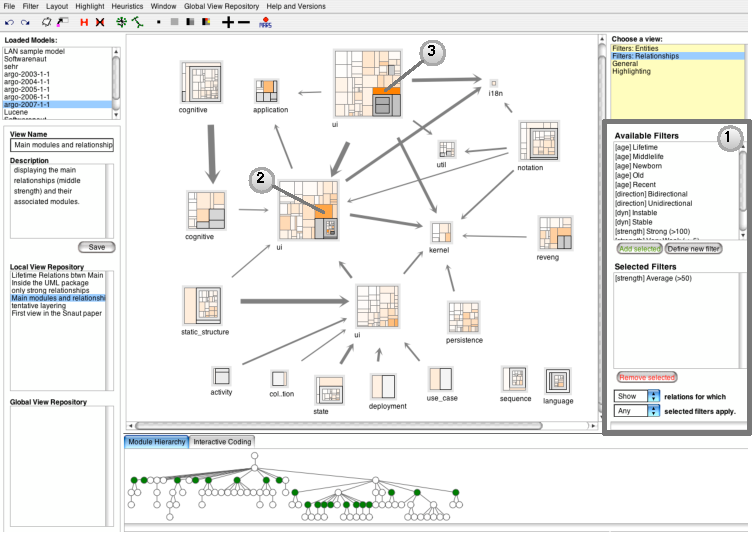
\includegraphics[width=\linewidth]{SnautFilteringPanel}
\caption{The UI for applying relationship filters in Softwarenaut}
\flabel{filpan}
\end{center}
\end{figure}

\fref{filpan} presents the relation filtering panel as implemented in Softwarenaut. Several filters can be combined to obtain more powerful ones with either the ``and'' or the ``or'' operator. The elements that match the filter can be either ``shown'' or ``hidden''. The user can define new filters by writing simple scripts in Smalltalk. The system is fully reflective, and as soon as a new filter is defined, it will immediately appear in the list of available filters.

Rule-based relationships are a powerful way of reducing information in the view. The principle is simple: not all the relationships are equally relevant for the task at hand. When analyzing a system with a specific goal, the analysis focuses first on those relationships that are most relevant for the chosen goal. Two different goals are architecture recovery and architecture quality assessment: 

\begin{itemize}

\item {\em Architecture Recovery.} When recovering the architecture of a system, the lifetime relationships are more relevant. They represent the architectural backbone of the system and their stability over time insures that it is worth analyzing them first.

\item {\em Architectural Quality Assessment.} When assessing the quality of an architecture, the recent relationships are of higher interest. Since they were recently introduced, they are more likely to be contrary to the original intended architecture. They might be the result of architectural decay or of changes to the system performed by new developers that are unaware of the architecture. Continuously monitoring these relationships can be a good quality assurance policy.
\end{itemize}



\fref{lvr} presents two views on the same modules that are also present in \fref{filpan} but with age-based filters activated. 

\begin{figure}[ht]
\begin{center}
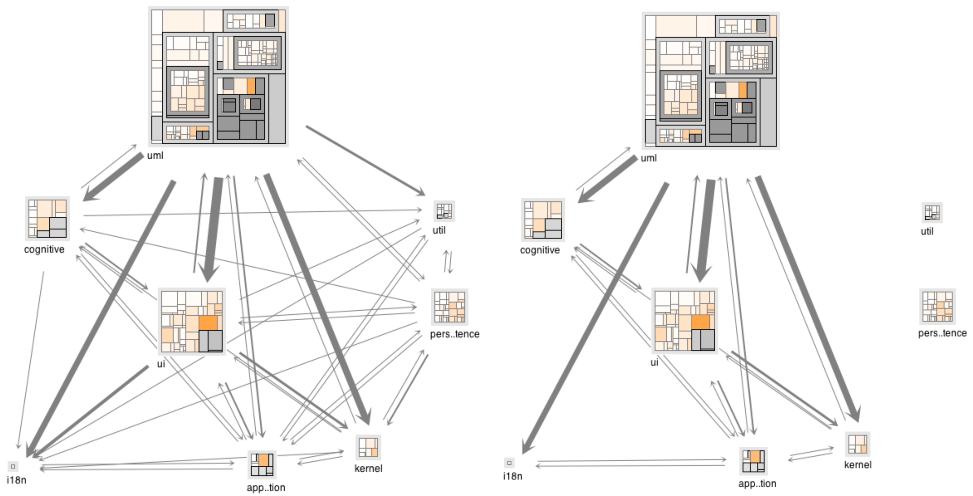
\includegraphics[width=\linewidth]{Architecture-LifetimeVsRecent}
\caption{The left part of the figure shows the Lifetime Relationships while the right part of the figure presents the Recent Relationships in Azureus/Vuze}
\flabel{lvr}
\end{center}
\end{figure}

The left side presents only the Lifetime Relationships - 21 relationships that existed between the displayed modules in all the versions of the system. The right side presents only the Recent Relationships - 36 relationships introduced in the system in the latest version. Both the numbers are very low in comparison with the total number of relationships that are present in the last version of the system; both function as powerful filters.

\newpage
\subsection {First-Class Views and Collaboration}
\slab{views}

The designers of a system use multiple diagrams for the specification of the architecture of a system. Also the reverse engineers need to recover multiple views when trying to understand the architecture of the system. To avoid information overload, architecture recovery tools usually support some kind of semantic zooming \cite{storey-shrimp}. We address this problem by directing the analysis towards the recovery of multiple architectural views. 

Views are first-class entities in Softwarenaut: one can save and restore any view during the exploration. This this allows for a {\em divide et impera} approach to architecture recovery and representation: each time a view risks becoming too complex the user saves it and the further exploration focuses only on a sub-part of the view. Moreover, views can be shared with other reverse architects.

View persistence requires the following information: The name and version of the system under analysis, the current working set with the positions of all the nodes in it, the active node and edge filters (both explicit and rule based), the creator of the view, and a name and description of the view. The model of the system is not saved together with the view. We assume that model construction is deterministic and the name and version of the system will suffice for model reconstruction at a later time \footnote{This requires nevertheless a way of uniquely identifying the entities in the view. In our case, for each of the entities in the working set we save the fully scoped name}.



% Moreover, in most of the cases the views are reused locally.


%The filters are predefined. In the future we plan to support user-defined filters and their publication together with the views. 


% \fref{viops} highlights the way the user can interact with the local views. He has a set of local views that he can save, load, delete locally. 

%\newpage
% COLLABORATION
%\section {Collaboration}
%\label {sec:collab}

% We have shown that in Softwarenaut views are entities that can be saved and restored. In this section we talk about the possibility of sharing the views with other users. 

Once published, a given version of a system never changes. It makes therefore sense to publish all the analyses regarding that version, such that when other users analyze the same version or system they can benefit from the previous work. In the context of architectural view recovery this means discovering architectural views that others have already defined. 


To support sharing architectural information we have created a {\em Global Architectural View Repository} (GVR) -- a public repository that indexes architectural views generated with Softwarenaut. The GVR is implemented as a relational database in PostgreSQL which can be publicly accessed by instances of Softwarenaut or other tools. %In the future we plan to provide a web services interface to the GVR. 

The architectural views as saved in the GVR can serve as the basis for monitoring the future architectural evolution of the system. After the publication of a new version of the system, Softwarenaut can automatically detect the views affected by the new changes, and present a {\em visual diff} on top of the view retrieved from the GVR between the state of the system at the moment the view was created and the latest commit.



\fref{viops} presents several considerations regarding the interaction with the architectural views in Sofwarenaut: 

\begin{itemize}

\item As soon as a user starts the analysis of a given system Softwarenaut checks the available view repositories and retrieves the list of views that are already defined for that system and/or version.

\item The top part of the inset presents the locally stored views which the user has in the image. For each of them the user can load it, delete it, or push it to the GVR. In the inset, the buttons which have black text represent operations that can be applied on the local views.

\item The bottom part presents the views which exist for the given system in the GVR. From the global view repository he can pull views in the local repository, or if he is the creator of such a view he can delete it from the global repository too. The view sharing mechanism is the latest addition to Softwarenaut.
\end{itemize}


\begin{figure}[h]
\begin{center}
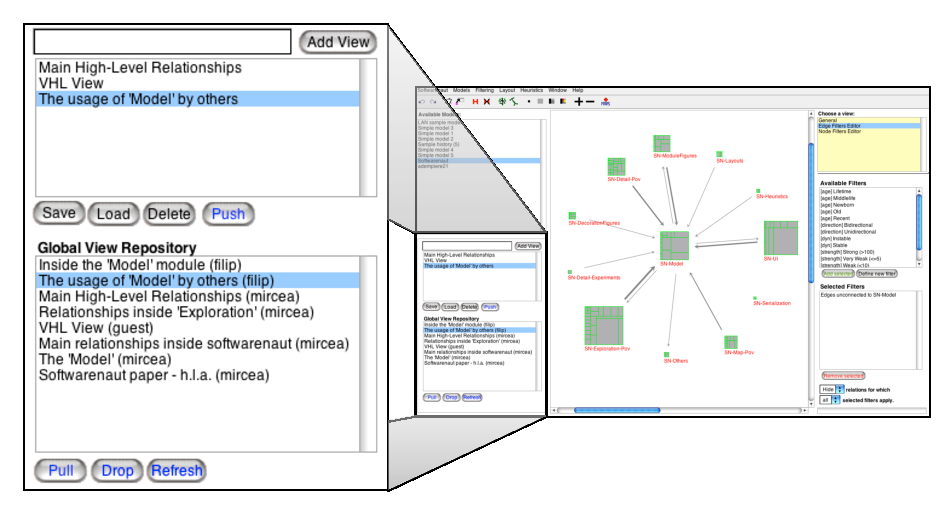
\includegraphics[width=\linewidth]{ViewOperations}
\caption{Views are first-class entities in Softwarenaut. They can be saved, deleted locally, but also published and retrieved from the Global Architectural View Repository.}
\flabel{viops}
\end{center}
\end{figure}







% In such a case SPO allows navigating down to the architectural level of the individual system, where it presents architectural views which are enriched with information from the ecosystem. 


\newpage
\section {Architectural Considerations Regarding Softwarenaut}
\slab{archi}


%%%%%%%%%%%%%%%%%%%%%%%%%%%%%%%%%%%%%
%%%%%%%%%%%%%%%%%%%%%%%%%%%%%%%%%%%%%
\subsection {Fact Extraction and Modelling} \label{sec:facts}
%%%%%%%%%%%%%%%%%%%%%%%%%%%%%%%%%%%%%
%%%%%%%%%%%%%%%%%%%%%%%%%%%%%%%%%%%%%

At the lowest level, Softwarenaut models a system using the Core of the FAMIX meta-model \cite{tichelaar-thesis}, a language independent meta-model that describes the static structure of object-oriented software systems. 
Given that the FAMIX meta-model is language independent, Softwarenaut can analyze any system written in an object-oriented language. This requires fact extractors that analyze the source code and build the intermediary FAMIX model. For this we use various third-party tools like McC \cite{pepi-mcc} or inFusion\footnote{See \url{http://www.intooitus.com/inFusion}, verified Jan 25 2011.}.

%%%%%%%%%%%%%%%%%%%%%%%%%%%%%%%%%%%%%
%{\bf Entities and relationships in FAMIX.}
%%%%%%%%%%%%%%%%%%%%%%%%%%%%%%%%%%%%%
FAMIX represents both artifacts and relationships as first-class entities. The main artifacts are namespaces, packages, classes, attributes, methods, fields. The main relationships between these entities are method invocations, variable accesses, class inheritances, and package include relationships \cite{tichelaar-thesis}.

A class of relationships which have a special importance in Softwarenaut are the containment relationships which organize a software system in a vertical hierarchy: classes contain methods, modules contain classes, systems contain modules. This containment mechanism is a powerful way of coping with the complexity of large software systems.

At an architectural level, different languages provide different mechanisms for the hierarchical organization of the system. C/C++ developers use the directory structure to organize systems hierarchically; Java developers use the package hierarchy; Smalltalk developers use the bundles hierarchy, etc. 
When a hierarchical decomposition is not provided, we can automatically generate one using clustering techniques \cite{koschke-thesis}. We presented elsewhere an experiment with clustering the classes in a system based on natural language similarity\cite{Lung05a}.

%%%%%%%%%%%%%%%%%%%%%%%%%%%%%%%%%%%%%
%{\bf Language Independence.}
%%%%%%%%%%%%%%%%%%%%%%%%%%%%%%%%%%%%%


\subsection {Integration with the Moose Analysis Platform}
We built Softwarenaut on top of the Moose Analysis Platform \cite{nier-story}. The main feature that the tool uses from Moose is the FAMIX Core meta-model for representing object-oriented systems. 
Softwarenaut makes uses of several of the views defined in Moose for the detail panel (e.g. the views that present entity metrics). Also, since behind any visual element of Softwarenaut lays a HiNode and behind it there is a FAMIX entity one can spawn other Moose analyses by selecting any of the elements of a Softwarenaut architectural view. In the same time, any tool in the Moose platform can spawn a Softwarenaut architectural analysis on any group of entities which have containment relationships and dependencies between themselves.


% The reliance of Softwarenaut on the FAMIX Core meta-model allows it to be independent of the programming language and analyze systems written in any language as long as there is a fact-extractor for that particular language. 



\subsection {Softwarenaut Synergies}
One of the tools that benefits from the Global View Repository is the Small Project Observatory (SPO), an ecosystem analysis tool that we have introduced elsewhere \cite{lungu-est}. SPO works at an abstraction level above the architectural level of individual systems: the {\em ecosystem abstraction level} \cite{lungu-thesis}. 

\begin{figure}[ht]
\begin{center}
\includegraphics[width=\linewidth]{SpoArchitectural}
\caption{SPO imports architectural views saved in Softwarenaut}
\label{}
\end{center}
\end{figure}
% This type of view is dynamic, it can not become obsolete...

% The main use case in which this navigation is needed is when one wants to understand a given system in the context of the ecosystem. 

SPO needs to support navigation between the two abstraction levels to support the understanding of  the ecosystem abstraction level. When navigating from the ecosystem abstraction level down to the architectural level SPO must present architectural views of the individual systems. When they are available, the architectural views of the individual systems are obtained from the Global View Repository. SPO can therefore reuse architectural information generated with Softwarenaut.

\subsection {History Operations} Softwarenaut keeps a history of the exploration and filtering actions to support undo and redo operations. This is a requirement for information exploration tools \cite{shneid-eyes} that few other architecture recovery tools implement.


% \newpage
% DISC
\section {Tool-Building Considerations}
\label {sec:disc}

Softwarenaut served as the research prototype for many of the research ideas we had during the PhD of the first author. As a result, the tool was the basis for a number of research papers \cite{lungu-cutedge, lungu-clust, lungu-packages, lungu-relevo}. Many of these papers could have not been written if it were not for the Softwarenaut which was a testbed for our ideas. 

We have obviously used Softwarenaut to to analyze Softwarenaut itself, and this has determined several re-architecting sessions. However, all throughout the development of the tool we wanted to have a tool that was usable. This allowed us to collaborate with others. We have integrated the tool with others \cite{lungu-clust, lungu-scico, nier-story} and we provided a framework in which masters projects to be developed \cite{boeckmann-mars}. We have also used the tool several times to perform reverse engineering in consulting projects.

In the next section we present a brief discussion on evaluating the tool with students.

\subsection {Evaluating the Usability and Usefulness of the Tool}
We have tested the Softwarenaut tool with students in the Software Evolution master course at the University of Lugano. In a qualitative experiment we asked the students to analyze a large software system \footnote{In this case it was ArgoUML} they have never seen before with the help of Softwarenaut and to produce an architectural report. Our goal in organizing the experiment was to test Softwarenaut and get feedback on both the usability of the tool and its usefulness for architecture recovery in the context of large software systems. 



To make the assignment more engaging for the students we grouped them in teams of two. To guide their analysis we asked them to perform a series of tasks which are presented in \fref{tasks}. After the students submitted the reports, we analyzed them ourselves and found them to be of various detail and quality. We list here several of the observations that we made after analyzing the reports that the students submitted:

\begin{figure}[t]
\begin{center}
\includegraphics[width=\linewidth]{tasks}
\caption{The eight tasks the students had to solve during two hours of the software design and evolution lab}
\flabel{tasks}
\end{center}
\end{figure}


\begin{itemize}
\item At question 1 that every group came with a different perspective and with a set of different views on the system. We considered this to be an argument for architecture being ``{\em is in the eye of the beholder}'' just as quality \cite{bass-architecture}.

\item The opinions were divided for question 2 and 3. Each group was ready to argue its position. 

\item Questions 4, 5, and 6 were not solved by everybody. We think the reason was the lack of sufficient training with the tool as well as some of the limitations that the users reported and which we present later.

\item All the groups that answered thought the system was well structured, fact with which we agree. However, one group blamed information overload for not answering. 

\end{itemize}

We also asked the students to fill a post-analysis questionnaire. 

By analyzing the post-experiment questionnaire we observed that most of the students found the tool easy to use and most of them considered that the reports they generated were reliable. They estimated that they got a better understanding of the system by using Softwarenaut. The most important feedback for us was related to the features of the tool that they students found useful, or the ones that they wanted to have but did not have:

\begin{itemize}
\item The features that the students found most useful in their analysis were the details-on-demand views, and the predefined filters for both nodes and edges.
\item The features that the students thought were missing (in decreasing order of the frequency of request) were: undo and redo facilities, user-defined filters, arbitrary and rule-based grouping of elements, view persistence.

\end{itemize}

Since then we have implemented most of the features that the students requested. One of these features is the view persistence and sharing as a means of supporting collaboration. In the future we plan to perform usability experiments that will evaluate the usability and usefulness of collaboration in architecture recovery and its implementation in the GVR by running some more controlled experiments.



\subsection {Depending on other research prototypes}
Depending on other research prototypes and platforms has been a benefit because we had the opportunity of using cutting edge technology, and building on the shoulders of giants, and in the same time, it made our life harder since the tools that we depended on kept moving ``under our feet'' and at times they were not maintained anymore. We believe however that the benefits outweighted the difficulties.


\subsection {Installation and Documentation}
Softwarenaut is written in the Smalltalk programming language and is released under the open source MIT Licence. The tool is available online at {\footnotesize \url{http://www.inf.usi.ch/phd/lungu/softwarenaut/}}. On the homepage of the tool there are a set of screencasts that present its various features together with other documentation, installation instructions, and instructions on how to obtain the source code. 


\newpage
% REL
\section {Related Work}
\label {sec:rel}

There is an extended tradition of architecture recovery tools in software engineering research. Pollet et al. have presented a comprehensive overview of the work in architecture recovery in their survey article \cite{pollet-sar}. In this section we take several of the core aspects of Softwarenaut and we discuss how they are similar and how they differ from other state of the art tools.

\subsection {Exploration and Navigation} 

The first architectural visualization prototype was Rigi, a programmable reverse engineering environment which emphasizes visualization and interaction \cite{muller-revengenv}. Rigi can visualize the data as hierarchical typed graphs and provides a Tcl interpreter for manipulating the graph data. The reconstruction process is based on a bottom-up process of grouping the software elements into clusters by manually selecting the nodes and collapsing them. The approach does not scale when analyzing very large systems because the number of low-level artifacts is too large. This is why in Softwarenaut we automatically aggregating the low-level relations, and then letting the user navigate from the highest abstraction level downwards is the main interaction approach in Softwarenaut. 

One of the projects that was inspired by Rigi was the SHriMP tool \cite{storey-shrimp} and its Eclipse-based continuation \cite{lintern-creole}. SHriMP and Creole display architectural diagrams using nested graphs. Their user interface embeds source code inside the graph nodes and integrates a hypertext metaphor for following low-level dependencies with animated panning, zooming, and fisheye-view ac- tions for viewing high-level structures.
The difference between our tool and Creole is that Softwarenaut can also perform evolutionary analysis.

Pinzger proposed the ArchView approach \cite{pinzger-thesis} which provides visualizations that present the evolution of the modules in a system. His evolution analysis takes into account the annotations from the versioning system repository. However, there is no support for first-class views in ArchView and the dependencies between the modules are only based on logical coupling. 


\subsection {Filtering}
 
%Most of the architecture recovery tools support filtering \cite{aracic-filtering}. The majority of the tools allow for the explicit filtering of individual relations. 

As far as we are aware we are the only ones to propose filters based on evolutionary aspects of the relationships in the context of software exploration. However, there are two related works. The first is Wierda et al. who recover the architectural decomposition of a system through clustering; they observe that if they use for clustering only those dependencies that were in the system in both the first and the last versions, the decompositions are more precise \cite{wierda-clustering}; this observation supports our approach of using the lifetime relationships as more architecturally relevant than the other relationships. 

The second related work is of Abram Hindle et al. \cite{hindle-yarn} who introduce the YARN visualization prototype which animates the evolution of dependencies between the modules of a system. The main difference between our approach and theirs is that we work on a snapshot-based model and they work on a commit-based model. Their commit-based model is advantageous since they benefit from more detailed information about the system; the disadvantage is that the animation of all the commits is time consuming. They do not support a query mechanism for visualizing only special types of relations.


\subsection {First-Class Views and Collaboration} 

The work of Storey et al. on Shrimp also allows for saving and restoring views \cite{rayside-flow}. The views are saved inside a ``Filmstrip'' which is persistent. Through the intermediation of the filmstrips the users can restore exploration sessions or even share certain views. This type of information allows people that know about each other to share information by emailing the files. The advantage of the Global View Repository is that it allows for discovering information that other users have discovered and about which the analysis is not aware. 
%(http://www.thechiselgroup.org/shrimp_manual_filmstrip)


Relevant for the collaborative reverse engineering part of our work is the Churrasco work of D’Ambros et al. \cite{dambros-churrasco}. Churrasco supports software evolution modeling, visualization and analysis through a web interface. 
Through an example scenario they show that Churrasco allows for collaborative software evolution analysis, and they attribute this to the availability on the web of the tool. The collaboration happens by annotating the various elements in the views of Churrasco. However, their tool presents a set of predefined views and they are not that much architectural views but rather design-level views. 

One project developed with collaboration support as the main goal is the Jazz IDE of IBM \cite{hupfer-jazz}. The goal of the Jazz ``collaborative development environment'' is to enhance and enrich collaboration in small, informal software development teams. Jazz has several features to support awareness of team member activities in addition to screen sharing such as local history of chats that are anchored in the code providing therefore context to the discussions. The main difference between their work and ours is the goal of the project.





\newpage
% CONC
\section {Conclusions and Future Work}
\label {sec:conc}

In this article we presented Softwarenaut, our tool for architecture recovery. The tool allows the recovery of architectural views of a software system through interactive exploration. The tool supports the ``overview first, zoom and filter, and details on demand'' principle of information visualization. It provides powerful filtering mechanisms and the capacity of saving and sharing architectural views. The tool was the test-bed for a variety of research projects and is still serving us in our research and consulting practice. 

There are two main research directions in which we would like to bring Softwarenaut beyond architecture recovery:

\begin{description}

\item {\em Reengineering.}
One of the tools built on top of Softwarenaut is MARS: an automated architecture refactoring recommender tool \cite{boeckmann-mars}. The tool starts from a given Softwarenaut view and checks whether move operations applied on classes can improve the architecture of the system by increasing coupling and decreasing cohesion. Preliminary results show a good recall but a low precision of the  automated refactoring recommendations generated by MARS. In the future we plan to explore more the space of reengineering operations that can be performed on an architectural view.


\item {\em Monitoring Software Evolution.}
One of our future projects is exploring ways in which the recovered views can function as a live documentation of an evolving system. The Softwarenaut views are not simple pictures but instead they code relationships between the modules of the system. A view recovered for a given version of the system can function as a reference point for presenting the future evolution of the system. After the publication of a new version of the system, Softwarenaut can automatically detect the views affected by the new changes, and visualize these changes on them.

\end{description}


\vspace{0.5cm}
\footnotesize
{\bf Acknowledgements.} We would like to thank Fabrizio Perin and Oscar Nierstrasz for feedback on earlier drafts of this paper.



\newpage

\footnotesize
%% The Appendices part is started with the command \appendix;
%% appendix sections are then done as normal sections
%% \appendix

%% \section{}
%% \label{}

%% References
%%
%% Following citation commands can be used in the body text:
%% Usage of \cite is as follows:
%%   \cite{key}          ==>>  [#]
%%   \cite[chap. 2]{key} ==>>  [#, chap. 2]
%%   \citet{key}         ==>>  Author [#]

%% References with bibTeX database:

\bibliographystyle{model1-num-names}
%\bibliography{scg,thesis}


\begin{thebibliography}{43}
\expandafter\ifx\csname natexlab\endcsname\relax\def\natexlab#1{#1}\fi
\providecommand{\bibinfo}[2]{#2}
\ifx\xfnm\relax \def\xfnm[#1]{\unskip,\space#1}\fi
%Type = Article
\bibitem[{Lehman(1980)}]{lehman-softev}
\bibinfo{author}{M.~Lehman},
\newblock \bibinfo{title}{Programs, life cycles, and laws of software
  evolution},
\newblock \bibinfo{journal}{Proceedings of the IEEE} \bibinfo{volume}{68}
  (\bibinfo{year}{Sept. 1980}) \bibinfo{pages}{1060--1076}.
%Type = Article
\bibitem[{Ducasse and Pollet(2009)}]{Duca09c}
\bibinfo{author}{S.~Ducasse}, \bibinfo{author}{D.~Pollet},
\newblock \bibinfo{title}{Software architecture reconstruction: A
  process-oriented taxonomy},
\newblock \bibinfo{journal}{IEEE Transactions on Software Engineering}
  \bibinfo{volume}{35} (\bibinfo{year}{2009}) \bibinfo{pages}{573--591}.
%Type = Inproceedings
\bibitem[{Pollet et~al.(2007)Pollet, Ducasse, Poyet, Alloui, C\^impan, and
  Verjus}]{pollet-sar}
\bibinfo{author}{D.~Pollet}, \bibinfo{author}{S.~Ducasse},
  \bibinfo{author}{L.~Poyet}, \bibinfo{author}{I.~Alloui},
  \bibinfo{author}{S.~C\^impan}, \bibinfo{author}{H.~Verjus},
\newblock \bibinfo{title}{Towards a process-oriented software architecture
  reconstruction taxonomy},
\newblock in: \bibinfo{editor}{R.~Krikhaar}, \bibinfo{editor}{C.~Verhoef},
  \bibinfo{editor}{G.~Di~Lucca} (Eds.), \bibinfo{booktitle}{Proceedings of 11th
  European Conference on Software Maintenance and Reengineering (CSMR'07)},
  \bibinfo{publisher}{IEEE Computer Society}, \bibinfo{year}{2007}, pp.
  \bibinfo{pages}{137--148}. \bibinfo{note}{Best Paper Award}.
%Type = Article
\bibitem[{Perry and Wolf(1992)}]{perry-foundations}
\bibinfo{author}{D.~E. Perry}, \bibinfo{author}{A.~L. Wolf},
\newblock \bibinfo{title}{Foundations for the study of software architecture},
\newblock \bibinfo{journal}{SIGSOFT Softw. Eng. Notes} \bibinfo{volume}{17}
  (\bibinfo{year}{1992}) \bibinfo{pages}{40--52}.
%Type = Article
\bibitem[{Garlan et~al.(2009)Garlan, Allen, and Ockerbloom}]{garlan-mismatch}
\bibinfo{author}{D.~Garlan}, \bibinfo{author}{R.~Allen},
  \bibinfo{author}{J.~Ockerbloom},
\newblock \bibinfo{title}{Architectural mismatch: Why reuse is still so hard},
\newblock \bibinfo{journal}{IEEE Softw.} \bibinfo{volume}{26}
  (\bibinfo{year}{2009}) \bibinfo{pages}{66--69}.
%Type = Inproceedings
\bibitem[{Riva(2000)}]{riva-report}
\bibinfo{author}{C.~Riva},
\newblock \bibinfo{title}{Reverse architecting: An industrial experience
  report},
\newblock in: \bibinfo{booktitle}{WCRE '00: Proceedings of the Seventh Working
  Conference on Reverse Engineering (WCRE'00)}, \bibinfo{publisher}{IEEE
  Computer Society}, \bibinfo{address}{Washington, DC, USA},
  \bibinfo{year}{2000}, p.~\bibinfo{pages}{42}.
%Type = Inproceedings
\bibitem[{Jazayeri(2002)}]{jaza-archevo}
\bibinfo{author}{M.~Jazayeri},
\newblock \bibinfo{title}{On architectural stability and evolution},
\newblock in: \bibinfo{booktitle}{Reliable Software Technlogies-Ada-Europe
  2002.}, \bibinfo{publisher}{Springer}, \bibinfo{year}{2002}, pp.
  \bibinfo{pages}{304--315}.
%Type = Book
\bibitem[{Bass et~al.(1997)Bass, Clements, and Kazman}]{bass-architecture}
\bibinfo{author}{L.~Bass}, \bibinfo{author}{P.~Clements},
  \bibinfo{author}{R.~Kazman}, \bibinfo{title}{Software Architecture in
  Practice}, \bibinfo{publisher}{{Addison-Wesley Professional}},
  \bibinfo{year}{1997}.
%Type = Article
\bibitem[{Kruchten(1995)}]{kruchten-4plus}
\bibinfo{author}{P.~Kruchten},
\newblock \bibinfo{title}{The 4+1 view model of architecture},
\newblock \bibinfo{journal}{IEEE Softw.} \bibinfo{volume}{12}
  (\bibinfo{year}{1995}) \bibinfo{pages}{42--50}.
%Type = Book
\bibitem[{Hofmeister et~al.(2000)Hofmeister, Nord, and Soni}]{hof-apparch}
\bibinfo{author}{C.~Hofmeister}, \bibinfo{author}{R.~Nord},
  \bibinfo{author}{D.~Soni}, \bibinfo{title}{Applied Software Architecture},
  \bibinfo{publisher}{Addison-Wesley}, \bibinfo{year}{2000}.
%Type = Inproceedings
\bibitem[{Murphy et~al.(1995)Murphy, Notkin, and Sullivan}]{murphy-reflexion}
\bibinfo{author}{G.~Murphy}, \bibinfo{author}{D.~Notkin},
  \bibinfo{author}{K.~Sullivan},
\newblock \bibinfo{title}{Software reflexion models: Bridging the gap between
  source and high-level models},
\newblock in: \bibinfo{booktitle}{Proceedings of SIGSOFT '95, Third ACM SIGSOFT
  Symposium on the Foundations of Software Engineering},
  \bibinfo{publisher}{ACM Press}, \bibinfo{year}{1995}, pp.
  \bibinfo{pages}{18--28}.
%Type = Article
\bibitem[{Muller and Klashinsky(1988)}]{muller-rigi}
\bibinfo{author}{H.~Muller}, \bibinfo{author}{K.~Klashinsky},
\newblock \bibinfo{title}{Rigi: a system for programming-in-the-large},
\newblock \bibinfo{journal}{Software Engineering, 1988., Proceedings of the
  10th International Conference on}  (\bibinfo{year}{1988})
  \bibinfo{pages}{80--86}.
%Type = Inproceedings
\bibitem[{Storey and M{\"u}ller(1995)}]{storey-shrimp}
\bibinfo{author}{M.-A.~D. Storey}, \bibinfo{author}{H.~A. M{\"u}ller},
\newblock \bibinfo{title}{Manipulating and documenting software structures
  using {SHriMP} {Views}},
\newblock in: \bibinfo{booktitle}{Proceedings of ICSM '95 (International
  Conference on Software Maintenance)}, \bibinfo{publisher}{IEEE Computer
  Society Press}, \bibinfo{year}{1995}, pp. \bibinfo{pages}{275--284}.
%Type = Inproceedings
\bibitem[{Lungu and Lanza(2007)}]{lungu-relevo}
\bibinfo{author}{M.~Lungu}, \bibinfo{author}{M.~Lanza},
\newblock \bibinfo{title}{Exploring inter-module relationships in evolving
  software systems},
\newblock in: \bibinfo{booktitle}{Proceedings of CSMR 2007 (11th European
  Conference on Software Maintenance and Reengineering)},
  \bibinfo{publisher}{IEEE Computer Society Press}, \bibinfo{address}{Los
  Alamitos CA}, \bibinfo{year}{2007}, pp. \bibinfo{pages}{91--100}.
%Type = Inproceedings
\bibitem[{Lungu et~al.(2006)Lungu, Lanza, and G\^irba}]{lungu-packages}
\bibinfo{author}{M.~Lungu}, \bibinfo{author}{M.~Lanza},
  \bibinfo{author}{T.~G\^irba},
\newblock \bibinfo{title}{Package patterns for visual architecture recovery},
\newblock in: \bibinfo{booktitle}{Proceedings of CSMR 2006 (10th European
  Conference on Software Maintenance and Reengineering)},
  \bibinfo{publisher}{IEEE Computer Society Press}, \bibinfo{address}{Los
  Alamitos CA}, \bibinfo{year}{2006}, pp. \bibinfo{pages}{185--196}.
%Type = Incollection
\bibitem[{Harel(1995)}]{harel-visform}
\bibinfo{author}{D.~Harel},
\newblock \bibinfo{title}{On visual formalisms},
\newblock in: \bibinfo{editor}{J.~Glasgow}, \bibinfo{editor}{N.~H. Narayanan},
  \bibinfo{editor}{B.~Chandrasekaran} (Eds.), \bibinfo{booktitle}{Diagrammatic
  Reasoning}, \bibinfo{publisher}{The {MIT} Press},
  \bibinfo{address}{Cambridge, Massachusetts}, \bibinfo{year}{1995}, pp.
  \bibinfo{pages}{235--271}.
%Type = Inproceedings
\bibitem[{Shneiderman(1996)}]{shneid-eyes}
\bibinfo{author}{B.~Shneiderman},
\newblock \bibinfo{title}{The eyes have it: {A} task by data type taxonomy for
  information visualizations},
\newblock in: \bibinfo{booktitle}{IEEE Visual Languages},
  \bibinfo{address}{College Park, Maryland 20742, U.S.A.}, pp.
  \bibinfo{pages}{336--343}.
%Type = Article
\bibitem[{Lanza and Ducasse(2003)}]{lanza-pv}
\bibinfo{author}{M.~Lanza}, \bibinfo{author}{S.~Ducasse},
\newblock \bibinfo{title}{Polymetric views - a lightweight visual approach to
  reverse engineering},
\newblock \bibinfo{journal}{Software Engineering, IEEE Transactions on}
  \bibinfo{volume}{29} (\bibinfo{year}{2003}) \bibinfo{pages}{782--795}.
%Type = Book
\bibitem[{Lanza and Marinescu(2006)}]{lanza-oomp}
\bibinfo{author}{M.~Lanza}, \bibinfo{author}{R.~Marinescu},
  \bibinfo{title}{Object-Oriented Metrics in Practice},
  \bibinfo{publisher}{Springer-Verlag}, \bibinfo{year}{2006}.
%Type = Phdthesis
\bibitem[{Wong(2000)}]{wong-thesis}
\bibinfo{author}{K.~Wong}, \bibinfo{title}{The reverse engineering notebook},
  Ph.D. thesis, University of Victoria, \bibinfo{address}{Victoria, B.C.,
  Canada, Canada}, \bibinfo{year}{2000}.
%Type = Inproceedings
\bibitem[{Storey et~al.(2005)Storey, \v{C}ubrani\'{c}, and
  German}]{storey-awareness}
\bibinfo{author}{M.-A.~D. Storey}, \bibinfo{author}{D.~\v{C}ubrani\'{c}},
  \bibinfo{author}{D.~M. German},
\newblock \bibinfo{title}{On the use of visualization to support awareness of
  human activities in software development: a survey and a framework},
\newblock in: \bibinfo{booktitle}{SoftVis '05: Proceedings of the 2005 ACM
  symposium on Software visualization}, \bibinfo{publisher}{ACM},
  \bibinfo{address}{New York, NY, USA}, \bibinfo{year}{2005}, pp.
  \bibinfo{pages}{193--202}.
%Type = Inproceedings
\bibitem[{Robertson et~al.(1991)Robertson, Mackinlay, and
  Card}]{robertson-conetrees}
\bibinfo{author}{G.~G. Robertson}, \bibinfo{author}{J.~D. Mackinlay},
  \bibinfo{author}{S.~K. Card},
\newblock \bibinfo{title}{Cone trees: animated 3d visualizations of
  hierarchical information},
\newblock in: \bibinfo{booktitle}{CHI '91: Proceedings of the SIGCHI conference
  on Human factors in computing systems}, \bibinfo{publisher}{ACM Press},
  \bibinfo{address}{New York, NY, USA}, \bibinfo{year}{1991}, pp.
  \bibinfo{pages}{189--194}.
%Type = Article
\bibitem[{Mitchell and Mancoridis(2006)}]{mitchell-bunch}
\bibinfo{author}{B.~S. Mitchell}, \bibinfo{author}{S.~Mancoridis},
\newblock \bibinfo{title}{On the automatic modularization of software systems
  using the bunch tool},
\newblock \bibinfo{journal}{IEEE Trans. Softw. Eng.} \bibinfo{volume}{32}
  (\bibinfo{year}{2006}) \bibinfo{pages}{193--208}.
%Type = Inproceedings
\bibitem[{Lungu and Lanza(2006)}]{lungu-cutedge}
\bibinfo{author}{M.~Lungu}, \bibinfo{author}{M.~Lanza},
\newblock \bibinfo{title}{Softwarenaut: cutting edge visualization},
\newblock in: \bibinfo{booktitle}{SoftVis '06: Proceedings of the 2006 ACM
  symposium on Software visualization}, \bibinfo{publisher}{ACM},
  \bibinfo{address}{New York, NY, USA}, \bibinfo{year}{2006}, pp.
  \bibinfo{pages}{179--180}.
%Type = Techreport
\bibitem[{Aracic et~al.(2007)Aracic, Schaeffer, Mezini, and
  Osterman}]{aracic-filtering}
\bibinfo{author}{I.~Aracic}, \bibinfo{author}{T.~Schaeffer},
  \bibinfo{author}{M.~Mezini}, \bibinfo{author}{K.~Osterman}, \bibinfo{title}{A
  Survey on Interactive Grouping and Filtering in Graph-based Software
  Visualizations}, \bibinfo{type}{Technical Report}, Technische Universit{\"a}t
  Darmstadt, \bibinfo{year}{2007}.
%Type = Phdthesis
\bibitem[{Tichelaar(2001)}]{tichelaar-thesis}
\bibinfo{author}{S.~Tichelaar}, \bibinfo{title}{Modeling Object-Oriented
  Software for Reverse Engineering and Refactoring}, Ph.D. thesis, University
  of Bern, \bibinfo{year}{2001}.
%Type = Article
\bibitem[{Mihancea et~al.(2007)Mihancea, Ganea, Verebi, Marinescu, and
  Marinescu}]{pepi-mcc}
\bibinfo{author}{P.~F. Mihancea}, \bibinfo{author}{G.~Ganea},
  \bibinfo{author}{I.~Verebi}, \bibinfo{author}{C.~Marinescu},
  \bibinfo{author}{R.~Marinescu},
\newblock \bibinfo{title}{Mcc and mc\#: Unified c++ and c\# design facts
  extractors tools},
\newblock \bibinfo{journal}{Symbolic and Numeric Algorithms for Scientific
  Computing, International Symposium on} \bibinfo{volume}{0}
  (\bibinfo{year}{2007}) \bibinfo{pages}{101--104}.
%Type = Article
\bibitem[{Koschke(2002)}]{koschke-thesis}
\bibinfo{author}{R.~Koschke},
\newblock \bibinfo{title}{Atomic architectural component recovery for program
  understanding and evolution},
\newblock \bibinfo{journal}{Software Maintenance, 2002. Proceedings.
  International Conference on}  (\bibinfo{year}{2002})
  \bibinfo{pages}{478--481}.
%Type = Inproceedings
\bibitem[{Lungu et~al.(2005)Lungu, Kuhn, G\^irba, and Lanza}]{Lung05a}
\bibinfo{author}{M.~Lungu}, \bibinfo{author}{A.~Kuhn},
  \bibinfo{author}{T.~G\^irba}, \bibinfo{author}{M.~Lanza},
\newblock \bibinfo{title}{Interactive exploration of semantic clusters},
\newblock in: \bibinfo{booktitle}{3rd International Workshop on Visualizing
  Software for Understanding and Analysis (VISSOFT 2005)}, pp.
  \bibinfo{pages}{95--100}.
%Type = Article
\bibitem[{Nierstrasz et~al.(2005)Nierstrasz, Ducasse, and Girba}]{nier-story}
\bibinfo{author}{O.~Nierstrasz}, \bibinfo{author}{S.~Ducasse},
  \bibinfo{author}{T.~Girba},
\newblock \bibinfo{title}{The story of moose: an agile reengineering
  environment},
\newblock \bibinfo{journal}{SIGSOFT Softw. Eng. Notes} \bibinfo{volume}{30}
  (\bibinfo{year}{2005}) \bibinfo{pages}{1--10}.
%Type = Article
\bibitem[{Lungu et~al.(2009)Lungu, Lanza, G\^{\i}rba, and Robbes}]{lungu-est}
\bibinfo{author}{M.~Lungu}, \bibinfo{author}{M.~Lanza},
  \bibinfo{author}{T.~G\^{\i}rba}, \bibinfo{author}{R.~Robbes},
\newblock \bibinfo{title}{The small project observatory: Visualizing software
  ecosystems},
\newblock \bibinfo{journal}{EST special issue of the Science of Computer
  Programming}  (\bibinfo{year}{2009}).
%Type = Phdthesis
\bibitem[{Lungu(2009)}]{lungu-thesis}
\bibinfo{author}{M.~Lungu}, \bibinfo{title}{Reverse Engineering Software
  Ecosystems}, Ph.D. thesis, University of Lugano, \bibinfo{year}{2009}.
%Type = Inproceedings
\bibitem[{Lungu et~al.(2005)Lungu, Kuhn, G\^irba, and Lanza}]{lungu-clust}
\bibinfo{author}{M.~Lungu}, \bibinfo{author}{A.~Kuhn},
  \bibinfo{author}{T.~G\^irba}, \bibinfo{author}{M.~Lanza},
\newblock \bibinfo{title}{Interactive exploration of semantic clusters},
\newblock in: \bibinfo{booktitle}{3rd International Workshop on Visualizing
  Software for Understanding and Analysis (VISSOFT 2005)}, pp.
  \bibinfo{pages}{95--100}.
%Type = Article
\bibitem[{Lungu et~al.(2010)Lungu, Lanza, Girba, and Robbes}]{lungu-scico}
\bibinfo{author}{M.~Lungu}, \bibinfo{author}{M.~Lanza},
  \bibinfo{author}{T.~Girba}, \bibinfo{author}{R.~Robbes},
\newblock \bibinfo{title}{The small project observatory: Visualizing software
  ecosystems},
\newblock \bibinfo{journal}{Science of Computer Programming, Elsevier}
  \bibinfo{volume}{75} (\bibinfo{year}{2010}) \bibinfo{pages}{264--275}.
%Type = Techreport
\bibitem[{Boeckmann(2010)}]{boeckmann-mars}
\bibinfo{author}{A.~Boeckmann}, \bibinfo{title}{MARS - Modular Architecture
  Recommendation System}, \bibinfo{type}{Bachelor's thesis}, University of
  Lugano, \bibinfo{year}{2010}.
%Type = Inproceedings
\bibitem[{M\"{u}ller et~al.(1992)M\"{u}ller, Tilley, Orgun, Corrie, and
  Madhavji}]{muller-revengenv}
\bibinfo{author}{H.~A. M\"{u}ller}, \bibinfo{author}{S.~R. Tilley},
  \bibinfo{author}{M.~A. Orgun}, \bibinfo{author}{B.~D. Corrie},
  \bibinfo{author}{N.~H. Madhavji},
\newblock \bibinfo{title}{A reverse engineering environment based on spatial
  and visual software interconnection models},
\newblock in: \bibinfo{booktitle}{SDE 5: Proceedings of the fifth ACM SIGSOFT
  symposium on Software development environments}, \bibinfo{publisher}{ACM},
  \bibinfo{address}{New York, NY, USA}, \bibinfo{year}{1992}, pp.
  \bibinfo{pages}{88--98}.
%Type = Inproceedings
\bibitem[{Lintern et~al.(2003)Lintern, Michaud, Storey, and
  Wu}]{lintern-creole}
\bibinfo{author}{R.~Lintern}, \bibinfo{author}{J.~Michaud},
  \bibinfo{author}{M.-A. Storey}, \bibinfo{author}{X.~Wu},
\newblock \bibinfo{title}{Plugging-in visualization: experiences integrating a
  visualization tool with eclipse},
\newblock in: \bibinfo{booktitle}{SoftVis '03: Proceedings of the 2003 ACM
  symposium on Software visualization}, \bibinfo{publisher}{ACM},
  \bibinfo{address}{New York, NY, USA}, \bibinfo{year}{2003}, pp.
  \bibinfo{pages}{47--ff}.
%Type = Phdthesis
\bibitem[{Pinzger(2005)}]{pinzger-thesis}
\bibinfo{author}{M.~Pinzger}, \bibinfo{title}{ArchView - Analyzing Evolutionary
  Aspects of Complex Software Systems}, Ph.D. thesis, Vienna University of
  Technology, \bibinfo{year}{2005}.
%Type = Inproceedings
\bibitem[{Wierda et~al.(2006)Wierda, Dortmans, and
  Lou~Somers}]{wierda-clustering}
\bibinfo{author}{A.~Wierda}, \bibinfo{author}{E.~Dortmans},
  \bibinfo{author}{L.~Lou~Somers},
\newblock \bibinfo{title}{Using version information in architectural clustering
  - a case study},
\newblock in: \bibinfo{booktitle}{CSMR '06: Proceedings of the Conference on
  Software Maintenance and Reengineering}, \bibinfo{publisher}{IEEE Computer
  Society}, \bibinfo{address}{Washington, DC, USA}, \bibinfo{year}{2006}, pp.
  \bibinfo{pages}{214--228}.
%Type = Article
\bibitem[{Hindle et~al.(2007)Hindle, Jiang, Koleilat, Godfrey, and
  Holt}]{hindle-yarn}
\bibinfo{author}{A.~Hindle}, \bibinfo{author}{Z.~M. Jiang},
  \bibinfo{author}{W.~Koleilat}, \bibinfo{author}{M.~W. Godfrey},
  \bibinfo{author}{R.~C. Holt},
\newblock \bibinfo{title}{Yarn: Animating software evolution},
\newblock \bibinfo{journal}{Visualizing Software for Understanding and
  Analysis, International Workshop on} \bibinfo{volume}{0}
  (\bibinfo{year}{2007}) \bibinfo{pages}{129--136}.
%Type = Article
\bibitem[{Rayside et~al.(2003)Rayside, Litoiu, Storey, Best, and
  Lintern}]{rayside-flow}
\bibinfo{author}{D.~Rayside}, \bibinfo{author}{M.~Litoiu},
  \bibinfo{author}{M.-A. Storey}, \bibinfo{author}{C.~Best},
  \bibinfo{author}{R.~Lintern},
\newblock \bibinfo{title}{Visualizing flow diagrams in websphere studio using
  shrimp views},
\newblock \bibinfo{journal}{Information Systems Frontiers} \bibinfo{volume}{5}
  (\bibinfo{year}{2003}) \bibinfo{pages}{161--174}.
  \bibinfo{note}{10.1023/A:1022649506310}.
%Type = Inproceedings
\bibitem[{D'Ambros and Lanza(2008)}]{dambros-churrasco}
\bibinfo{author}{M.~D'Ambros}, \bibinfo{author}{M.~Lanza},
\newblock \bibinfo{title}{A flexible framework to support collaborative
  software evolution analysis},
\newblock in: \bibinfo{booktitle}{Proceedings of CSMR 2008 (12th European
  Conference on Software Maintenance and Reengineering)},
  \bibinfo{publisher}{IEEE Computer Society}, \bibinfo{year}{2008}, pp.
  \bibinfo{pages}{3--12}.
%Type = Inproceedings
\bibitem[{Hupfer et~al.(2004)Hupfer, Cheng, Ross, and Patterson}]{hupfer-jazz}
\bibinfo{author}{S.~Hupfer}, \bibinfo{author}{L.-T. Cheng},
  \bibinfo{author}{S.~Ross}, \bibinfo{author}{J.~Patterson},
\newblock \bibinfo{title}{Introducing collaboration into an application
  development environment},
\newblock in: \bibinfo{booktitle}{Proceedings of the 2004 ACM conference on
  Computer supported cooperative work}, CSCW '04, \bibinfo{publisher}{ACM},
  \bibinfo{address}{New York, NY, USA}, \bibinfo{year}{2004}, pp.
  \bibinfo{pages}{21--24}.
\end{thebibliography}

%\
% Authors are advised to submit their bibtex database files. They are
%% requested to list a bibtex style file in the manuscript if they do
%% not want to use model1-num-names.bst.

%% References without bibTeX database:

% \begin{thebibliography}{00}

%% \bibitem must have the following form:
%%   \bibitem{key}...
%%

% \bibitem{}



\end{document}

%%
%% End of file `elsarticle-template-1-num.tex'.
